\chapter{Geometria Plana}
		\section{Triângulos}
		\begin{list}{\textbf{Questão \arabic{quest}.}}{\usecounter{quest}}
%define a margem da lista.	
%\setlength{\labelwidth}{-2mm} \setlength{\parsep}{0mm}
%\setlength{\topsep}{0mm} \setlength{\leftmargin}{-2mm}
\renewcommand{\labelenumi}{(\alph{enumi})}

		
			\item Diga se é possível construir um triângulo com lados cujas medidas são:
				\begin{enumerate}
					\item a = 8 cm, b = 6 cm e c = 5 cm
					\item a = 5 cm, b = 2 cm e c = 3 cm
					\item a = 5,4 cm, b = 1 cm e c = 3,5 cm
					\item a = 6,5 cm, b = 4,5 cm e c = 5 cm							
				\end{enumerate}
				
				\item Na figura ,med($\widehat{B}$) = $60^o$ e med($\widehat{C}$) = $40^o$. Se \textbf{D} é o \textbf{incentro} do triângulo ABC, então \textbf{x} vale:
				
				\begin{center}
				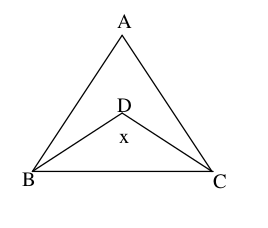
\includegraphics[scale=0.7]{figuras/fig28}
				\end{center}
				\begin{multicols}{5}
				\begin{enumerate}
					\item 120$^o$
					\item 130$^o$
					\item 150$^o$
					\item 100$^o$
					\item 40$^o$
				\end{enumerate}
				\end{multicols}
				
			\item Determine o valor dos termos desconhecidos nos triângulos abaixo:\\
			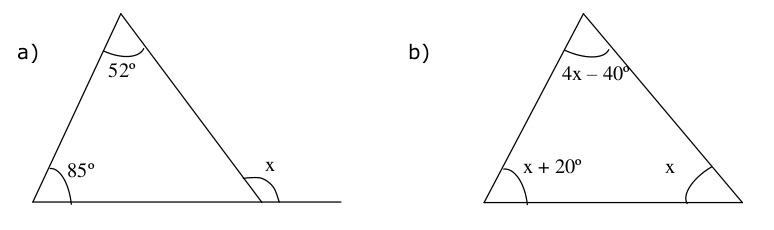
\includegraphics[scale=0.7]{figuras/fig26.png}\\
			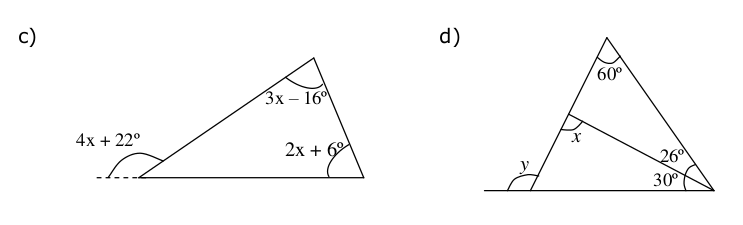
\includegraphics[scale=0.7]{figuras/fig27.png}
			
			\item Na figura, o $\bigtriangleup ABC$ é congruente ao $\bigtriangleup EDC$. Determine o caso de congruência e o valor de x e y.
			
			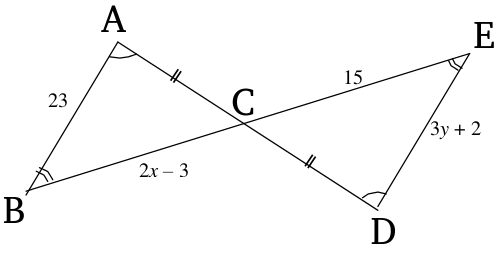
\includegraphics[scale=0.7]{figuras/fig29.png}
		\end{list}
		 \section{Congruência de Triângulo}	
		 	\begin{list}{\textbf{Questão \arabic{quest}.}}{\usecounter{quest}}
%define a margem da lista.	
%\setlength{\labelwidth}{-2mm} \setlength{\parsep}{0mm}
%\setlength{\topsep}{0mm} \setlength{\leftmargin}{-2mm}
\renewcommand{\labelenumi}{(\alph{enumi})}

		 		\item Os triângulos ABC e MNP são congruentes. Pelas indicações, determine o caso de congruências e as medidas x e y.	 		
		 		\begin{center}
		 		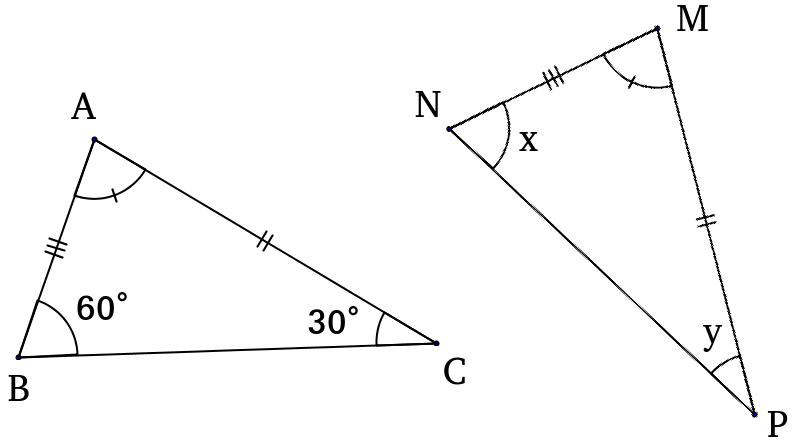
\includegraphics[scale=0.4]{figuras/fig17.png}
		 		\end{center}
		 		
		 		\item Na figura, $\widehat{B} \cong \widehat{E}$ e $\overline{AB} \cong \overline{DE}$. Nessas condições, determine as medidas de $x$ e $y$.		 		
		 		\begin{center}
		 		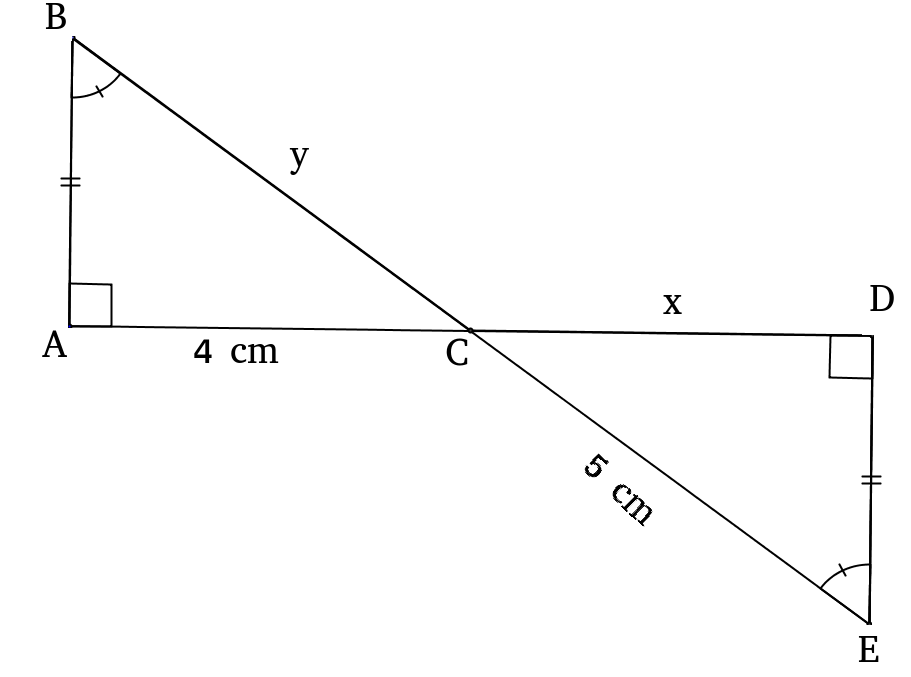
\includegraphics[scale=0.4]{figuras/fig18.png}
		 		\end{center}
		 		
		 		\item Na figura, prove que $\bigtriangleup ABC \cong \bigtriangleup CBD.$
		 		\begin{center}
		 		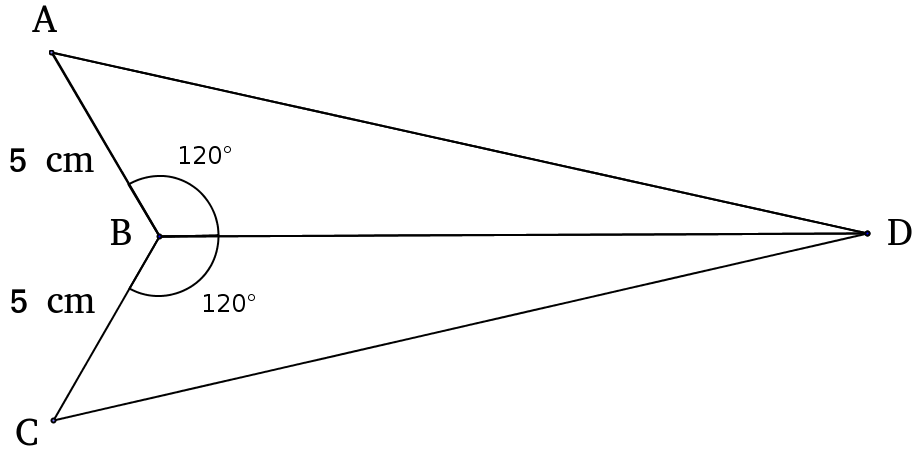
\includegraphics[scale=0.4]{figuras/fig19.png} 
		 		\end{center}
		 		
		 		\item Na figura, $\overline{AC} \cong \overline{MN}$ e $\widehat{C} \cong \widehat{N}$. Prove que $\overline{AB} \cong \overline{PM}$.
		 		\begin{center}
		 		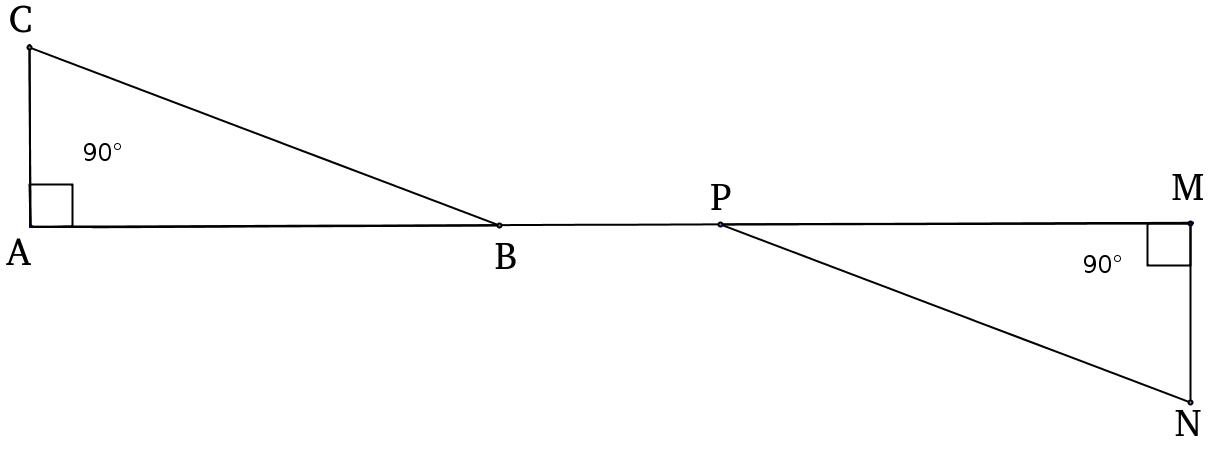
\includegraphics[scale=0.4]{figuras/fig20.png}
		 		\end{center}
		 		
		 		\item No $\bigtriangleup ABC, \overline{AB} \cong \overline{AC}$ e $\overline{BD} \cong \overline{DC}$. Nessas condições, mostre que:
		 		\begin{multicols}{3}
		 		\begin{enumerate}
		 			\item $x=y$.
		 			\item $\widehat{B} \cong \widehat{C}$.
		 			\item $\overline{AB}$ é altura do $\bigtriangleup ABC$.
		 		\end{enumerate}
		 		\end{multicols}
		 		
		 		\item (Saresp) Na figura, o triângulo ABC é isóceles e $\overline{BD} \cong \overline{DE} \cong \overline{EC}$. Nessas condições, os triângulos:
		 		\begin{enumerate}
		 			\item ABD e ADE são congruentes.
		 			\item ABD e AEC são congruentes.
		 			\item ADE e AEC são congruentes.
		 			\item ABD e ABC são congruentes.
		 		\end{enumerate}
		 		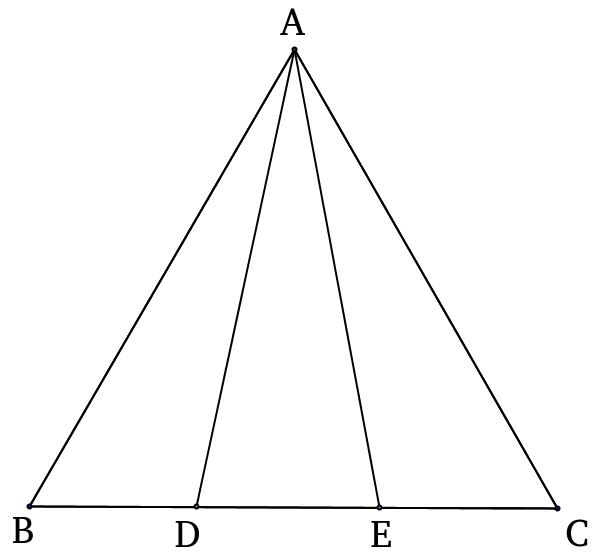
\includegraphics[scale=0.4]{figuras/fig21.png}
				
				\item Na figura, $\widehat{A} \cong \widehat{B}$ e $\overline{AM} \cong \overline{MB}$. Prove que $M$ é ponto médio de $\overline{CD}$.
				\begin{flushleft}
				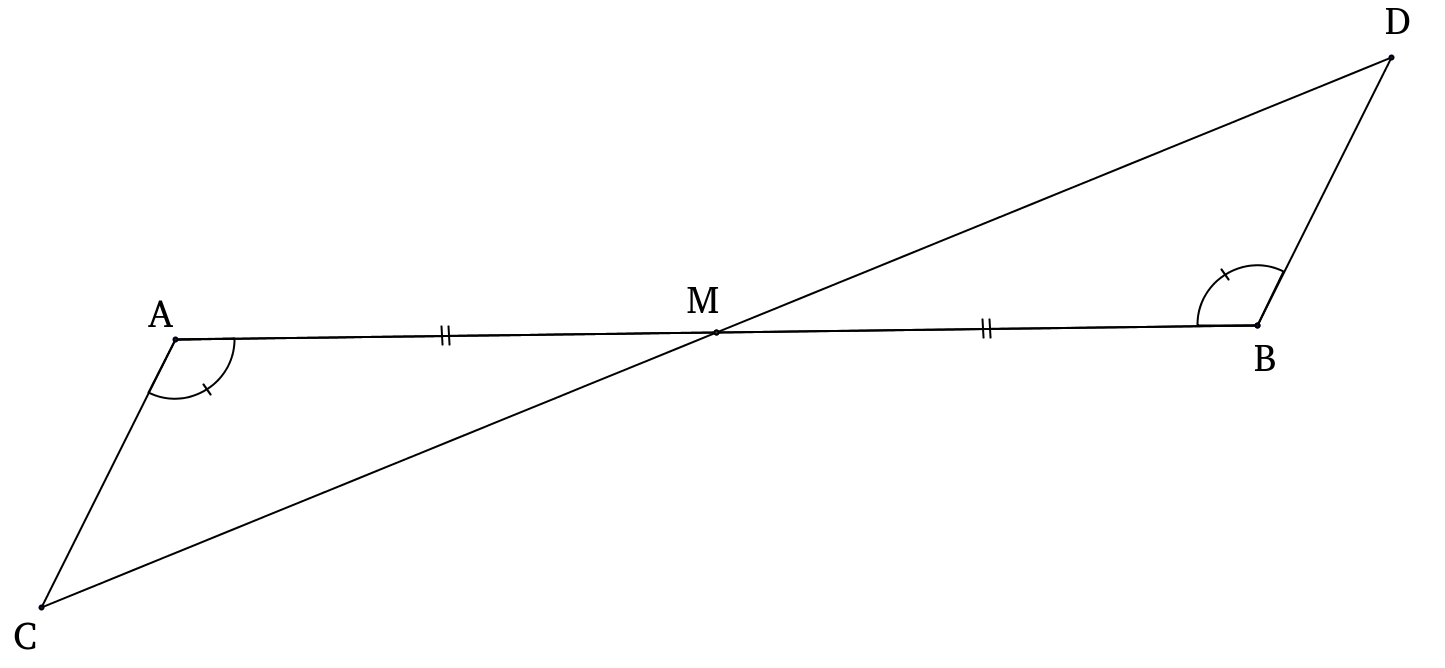
\includegraphics[scale=0.4]{figuras/fig22.png}
				\end{flushleft}
			\end{list}	
			
			\section{Quadriláteros}
			\begin{list}{\textbf{Questão \arabic{quest}.}}{\usecounter{quest}}
%define a margem da lista.	
%\setlength{\labelwidth}{-2mm} \setlength{\parsep}{0mm}
%\setlength{\topsep}{0mm} \setlength{\leftmargin}{-2mm}
\renewcommand{\labelenumi}{(\alph{enumi})}

				\item  Coloque (V) para verdadeiro e (F) para falso nas afirmativas abaixo:
				\begin{enumerate}
				\item ( \ ) As diagonais de um quadrado são sempre congruentes.
				\item ( \ ) As diagonais de um losango são sempre congruentes.
				\item ( \ ) As diagonais de um retângulo são sempre congruentes.
				\item ( \ ) As diagonais de um losango são sempre perpendiculares.
				\item ( \ ) Todo retângulo é um quadrado.
				\end{enumerate}
				
				\item Observe os paralelogramos e, considerando as propriedades estudadas, determine:
				\begin{multicols}{2}
				\begin{enumerate}
					\item MN e NP 
					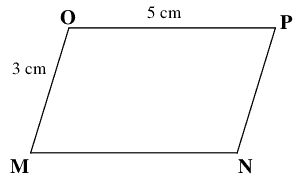
\includegraphics[scale=0.7]{figuras/fig30.png}
					\item x e y 
					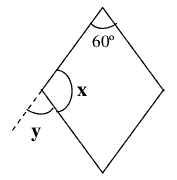
\includegraphics[scale=0.7]{figuras/fig31.png}
					\item $med(\widehat{A}),med(\widehat{B}),med(\widehat{C})$\\
					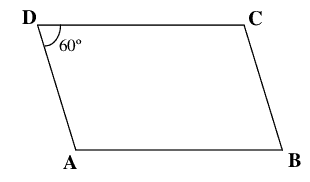
\includegraphics[scale=0.7]{figuras/fig32.png}
					\item O perímetro do triângulo RMS.
					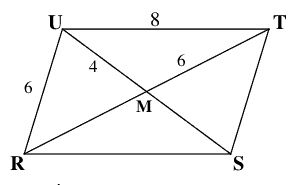
\includegraphics[scale=0.7]{figuras/fig33.png}
				\end{enumerate}
				\end{multicols}
				
				\item No retângulo ABCD da figura a seguir, M é ponto médio do lado CD. O valor da medida x indicada na figura abaixo é:
				\begin{center}
				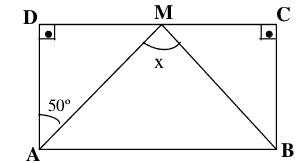
\includegraphics[scale=0.7]{figuras/fig34.png}
				\end{center}
				\begin{multicols}{5}
				\begin{enumerate}
					\item 50$^o$
					\item 45$^o$
					\item 100$^o$
					\item 75$^o$
					\item 80$^o$
				\end{enumerate}
				\end{multicols}
				
				\item Encontre os valores de x e y.
				\begin{multicols}{2}
				\begin{enumerate}
					\item ABCD é um losango
					\item[] 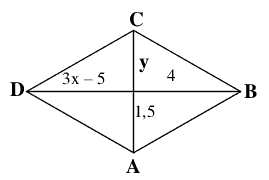
\includegraphics[scale=0.7]{figuras/fig35}
					\item ABCD é retângulo
					\item[] 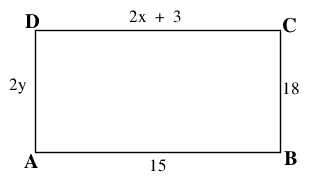
\includegraphics[scale=0.7]{figuras/fig36}
				\end{enumerate}
				\end{multicols}
				
				\item Observe o paralelogramo e determine:
				\begin{center}
				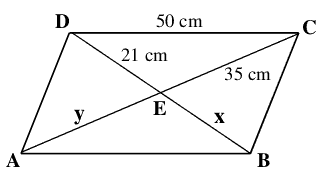
\includegraphics[scale=0.7]{figuras/fig37}
				\end{center}
				\begin{multicols}{2}
				\begin{enumerate}
					\item as medidas de x e Y indicadas.
					\item o perímetro do $\bigtriangleup ABC$
				\end{enumerate}
				\end{multicols}
				
				\item Calcula o valor de x e y nos trapézios abaixo.
				\begin{multicols}{2}
				\begin{enumerate}
					\item 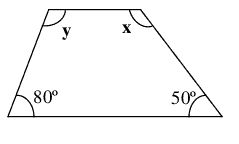
\includegraphics[scale=0.7]{figuras/fig38}
					\item 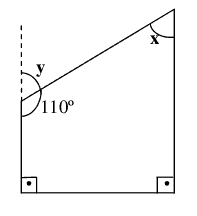
\includegraphics[scale=0.7]{figuras/fig39}
				\end{enumerate}
				\end{multicols}
				
				\item A figura abaixo é um trapézio isósceles. Sabendo que AM está contido na bissetriz do ângulo $\widehat{A}$ e BM está contido na bissetriz do ângulo $\widehat{B}$, o valor da medida x indicada é:
				\begin{center}
				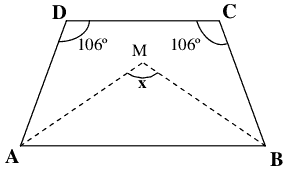
\includegraphics[scale=0.7]{figuras/fig40}
				\end{center}
				
				\begin{multicols}{4}
				\begin{enumerate}
					\item 74
					\item 36
					\item 104
					\item 106
				\end{enumerate}
				\end{multicols}
				
				\item No paralelogramo, temos: $med(\widehat{B}) = 80^o$, $\overline{BM}$ é bissetriz do $\widehat{A}$. Calcule a medida do ângulo $A\widehat{M}B$.
				
				\begin{center}
				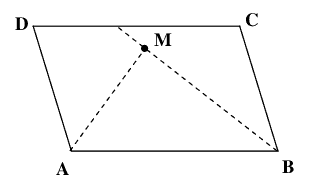
\includegraphics[scale=0.7]{figuras/fig41}
				\end{center}
			\end{list}

